\section{Reducing security to safety}\label{sec:body}

% Explain the paper, in your own words. Don't go into as many details as the
% original text, but the person reading your review should have a general
% understanding of the paper's results and how those results can be obtained.
% The structure and content of this section of course heavily depends on the
% paper itself. Don't hesitate to split it in multiple sections or subsections,
% for example: \subsection{An algorithm for whatever problem we try to solve} If
% your paper contains theorems, sketch the proofs of important theorems.

% \subsection{Benchmarks} If it contains benchmarks, show the key scores or
% results.

% You can follow the structure of the paper you're reviewing, but write with
% your own words.

% \subsection{Reducing security to safety}

% At the interface of any security-sensitive function call, there usually exists a
% \emph{contract} that describes which inputs or outpus are deemed public (i.e.,
% known to attackers) and which ones are private (i.e., to protect). A leak should
% never reveal anyting about the private inputs and outputs (but publics ones 
% can be leaked).
% If we denote a program as $p$ (with the usual definition of a prgram being a
% sequence of statements or programs) with a corresponding state $s$ (which
% is mapping from variables to values) then at each step of execution, from
% state $s$ executing program/statement $p$ we can define leakage $L(.)$ as follows:

% \begin{equation}
%     \begin{split}
%     L(\langle s, \text{\texttt{if}}~e~\text{\texttt{then}}~p_1~\text{\texttt{else}}~p_2 \rangle) = & s(e) \\
%     L(\langle s, \text{\texttt{while}}~e~\text{\texttt{do}}~p \rangle) = & s(e) \\
%     L(\langle s, x_0[e_0] = e \rangle) = & s(e_0)s(e_1)...s(e_n)
%     \end{split}
% \end{equation}

% The first two leakage sources correspond to leakage from control flow while the
% latter is leakage from memory access. Note that in the third leakage source,
% a memory leak $s(e_0)$ corresponds to leakage from the right-hand-side indexer
% expression and $s(e_1)$ to $s(e_n)$ possible indexer expression in expression
% $e$. We can also extend the leakage sources to comprise machine operations that
% have operand-dependent execution latency (i.e., division in x86).

We now illustrate (using an example) how the authors use the leakage rules in \secref{prelimnaries} 
to reduce constant-time security to assertion safety.

We use the program listed in \figref{example} as our running example. 
This program copies a sub-array of length \texttt{sub\_len}, starting at index \texttt{l\_idx}, from array \texttt{in}
to array \texttt{out}.
We assume that the starting addresses and lengths of both arrays are publicly observable but the value of \texttt{l\_idx} and the array contents must be kept a secret.
Note, this program is \emph{not constant-time secure} since the branches on line 5 clearly leak information about \texttt{l\_idx}.

\begin{figure}[h]
    \centering\resizebox{0.7\columnwidth}{!}{\lstinputlisting[language=C]{example.c}}
    \caption{Running example - sub-array copy}
    \label{fig:example}
\end{figure}


The authors reduce the constant-time security of the original program ($P$) to the assertion safety of a second program ($Q$) that is the \emph{self-product} of $P$.
Said differently, $Q$ is a program in which two abstract executions of $P$ take place simultaneously, with the two executions only differing in the value of \emph{secret} inputs and outputs. 
\figref{rules}~.a shows how such a self-product can be constructed ($\hat{p}$ is the program $p$ with all variables renamed).
First, each public input is assumed to be equal in both executions, then a guard and instrumentation are recursively applied to each subprogram. 
The guards assert the equality of leakage functions for each subprogram $p$ and its variable-renaming $\hat{p}$.
The essence of the transformation lies in the instrumentation (~\figref{rules}~.b) which reduces constant-time security to assertion safety. 
The authors formalize this reduction from constant-time security to safety in Coq and prove that it is sound for all safe input programs (i.e., a security verdict is always correct) and complete for programs where information about public outputs is not taken into consideration in the security analysis (i.e., an insecurity verdict is always correct).

\begin{figure}[h]
    \centering
    \subfigure[Program product construction rules]{
        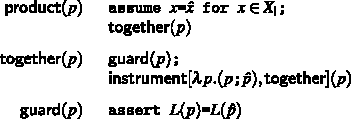
\includegraphics[width=0.45\textwidth]{./figs/fig_7.pdf}
    }\label{fig:fig_7}
    \subfigure[Instrumentation rules.] {
        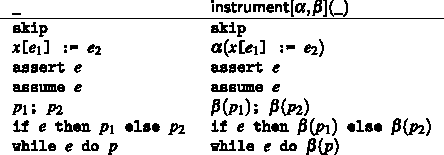
\includegraphics[width=0.45\textwidth]{./figs/fig_8.pdf}
    }\label{fig:fig_8}
    \caption{Program product}
    \label{fig:rules}
\end{figure}

\figref{example_prod} illustrates the self-product for our running example. 
The resultant program is instrumented with assertions to ensure leakage remains the same at
every step of execution.
Since \texttt{l\_idx} is a private input to the program, its renaming cannot be assumed equal.
Consequently, the assertion on line $8$ fails, demonstrating that assertions in the self-product do not hold if the given program does not run in constant time.

\begin{figure}[h]
    \centering\resizebox{0.9\columnwidth}{!}{\lstinputlisting[language=MySketch]{prod.c}}
    \caption{Example program product of the sub-array copy program.}
    \label{fig:example_prod}
\end{figure}